\chapter{Realisierung}\label{ch:realisierung}
In diesem Kapitel wird die tatsächliche Umsetzung der automatischen Datengenerierung für das \ac{CIF} thematisiert. Zunächst wird eine grundsätzliche Implementierung auf Basis des im vorangegangenen Kapitel beschriebenen Konzepts für die Equipment-Entität \enquote{Chassis} dargestellt. Das darauf folgende Unterkapitel \ref{sec:tdgmodule} beschäftigt sich mit der Erweiterung der Basisimplementierung zur Unterstützung von verschiedenen auch komplexeren Entitäten am Beispiel der Subequipment-Entität \enquote{Module}. Schließlich wird im Kapitel \ref{sec:tdgtelco} noch ein Konzept für eine mögliche künftige Implementierung von Telco-Entitäten, einer weiteren Komplexitätsstufe der Entitäten, vorgestellt.

\section{Realisierung der Testdatengenerierung für Equipment-Entitäten am Beispiel der Chassis}\label{sec:tdgchassis}


Es wurde sich für die Konfigurationsdateien für das \ac{CSV}-Format entschieden, da \ac{CSV}-Dateien in Programmen wie \textit{Microsoft Excel} in Tabellenform geöffnet und auch dort direkt bearbeitet werden können. \cite{excel:2022} So ist es möglich, die Konfigurationsdateien gleichzeitig gewissermaßen als Dokumentation zu verwenden, da sie auch beschreiben sollte, welche Deltafälle und Entitäten in der Datengenerierung umgesetzt sind.


\begin{lstlisting}[caption=Konfigurationsdatei für Deltafälle im CSV-Format, label=Delta-Spezifikationen,language=json]
    Delta Case;NMS Record;Command Record;Planned Create Record; Planned Delete Record
    CREATE;nms;;;
    UPDATE;nms;command;;
    DELETE;;command;;
    UPDATE_TYPE;nms;command;;
    PLANNED_CREATE;nms;;planningCreate;
    PLANNED_CREATE_NOP;;;planningCreate;
    PLANNED_CREATE_BUT_WITH_DIFFERENT_TYPE;nms;;planningCreate;
    PLANNED_DELETE;;command;;planningDelete
    PLANNED_DELETE_NOP;nms;command;;planningDelete
    PLANNED_DELETE_WITH_CREATE;nms;command;;planningDelete
    PLANNED_DELETE_WITH_PLANNED_CREATE_BUT_WITH_DIFFERENT_TYPE;nms;command;planningCreate;planningDelete
    PLANNED_DELETE_WITH_PLANNED_CREATE;nms;command;planningCreate;planningDelete
    PLANNED_DELETE_WITH_PLANNED_CREATE_NOP;nms;command;planningCreate;planningDelete
    PLANNED_DELETE_WITH_PLANNED_CREATE_NOP_DELETION;;command;planningCreate;planningDelete
    PRECOND;;command;;
\end{lstlisting}

\begin{figure}[h]
    \centering
    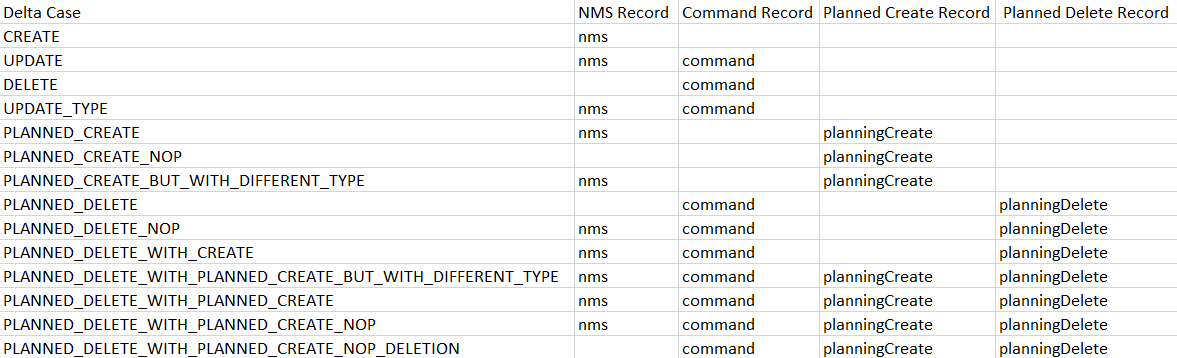
\includegraphics[width=\textwidth]{delta-specifications-excel.png}
    \caption{Konfigurationsdatei für Deltafälle in \textit{Excel}\footnotemark}
\end{figure}

Bisherige Struktur mit POJO-Klassen für alle Entitäten wurde als unpraktisch und kompliziert evaluiert und so wurde sich entschieden, für die generische Implementierung der Testdatengenerierung diese Struktur zu verwerfen und stattdessen eine zentrale Klasse zu entwerfen, welche alle möglichen Entitäten erfassen kann. Dies ist möglich, da für die Erstellung von Objekten über die BGEs die entsprechenden Objekte lediglich als \ac{JSON}-String im Body der REST-Anfrage gesendet werden müssen - speziell auf eine Entität angepasste Klassen sind also gar nicht vonnöten.

\section{Erweiterung der Testdatengenerierung für Subequipment-Entitäten am Beispiel der Module}\label{sec:tdgmodule}
Text

\section{Erarbeiten eines Konzepts zur Testdatengenerierung für Telco-Entitäten}\label{sec:tdgtelco}
Text